
\tikzset{every picture/.style={line width=0.75pt}} %set default line width to 0.75pt        

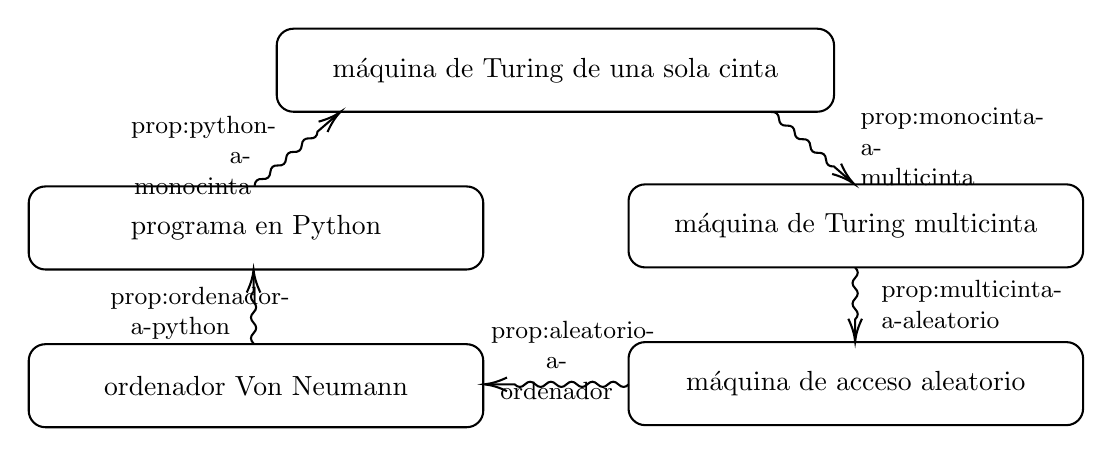
\begin{tikzpicture}[x=0.75pt,y=0.75pt,yscale=-1,xscale=1]
%uncomment if require: \path (0,489); %set diagram left start at 0, and has height of 489

%Rounded Rect [id:dp38098198089187774] 
\draw   (241,29) .. controls (241,24.58) and (244.58,21) .. (249,21) -- (501.5,21) .. controls (505.92,21) and (509.5,24.58) .. (509.5,29) -- (509.5,53) .. controls (509.5,57.42) and (505.92,61) .. (501.5,61) -- (249,61) .. controls (244.58,61) and (241,57.42) .. (241,53) -- cycle ;
%Rounded Rect [id:dp7442940701895104] 
\draw   (410.5,104) .. controls (410.5,99.58) and (414.08,96) .. (418.5,96) -- (621.5,96) .. controls (625.92,96) and (629.5,99.58) .. (629.5,104) -- (629.5,128) .. controls (629.5,132.42) and (625.92,136) .. (621.5,136) -- (418.5,136) .. controls (414.08,136) and (410.5,132.42) .. (410.5,128) -- cycle ;
%Rounded Rect [id:dp05734792720775661] 
\draw   (410.5,180) .. controls (410.5,175.58) and (414.08,172) .. (418.5,172) -- (621.5,172) .. controls (625.92,172) and (629.5,175.58) .. (629.5,180) -- (629.5,204) .. controls (629.5,208.42) and (625.92,212) .. (621.5,212) -- (418.5,212) .. controls (414.08,212) and (410.5,208.42) .. (410.5,204) -- cycle ;
%Rounded Rect [id:dp6203792922315816] 
\draw   (121.5,105) .. controls (121.5,100.58) and (125.08,97) .. (129.5,97) -- (332.5,97) .. controls (336.92,97) and (340.5,100.58) .. (340.5,105) -- (340.5,129) .. controls (340.5,133.42) and (336.92,137) .. (332.5,137) -- (129.5,137) .. controls (125.08,137) and (121.5,133.42) .. (121.5,129) -- cycle ;
%Rounded Rect [id:dp5638157358715545] 
\draw   (121.5,181) .. controls (121.5,176.58) and (125.08,173) .. (129.5,173) -- (332.5,173) .. controls (336.92,173) and (340.5,176.58) .. (340.5,181) -- (340.5,205) .. controls (340.5,209.42) and (336.92,213) .. (332.5,213) -- (129.5,213) .. controls (125.08,213) and (121.5,209.42) .. (121.5,205) -- cycle ;
%Straight Lines [id:da13357301440091862] 
\draw    (479.2,61.14) .. controls (481.55,60.97) and (482.81,62.06) .. (482.98,64.41) .. controls (483.14,66.76) and (484.4,67.86) .. (486.75,67.69) .. controls (489.1,67.52) and (490.36,68.62) .. (490.53,70.97) .. controls (490.7,73.32) and (491.96,74.41) .. (494.31,74.24) .. controls (496.66,74.07) and (497.92,75.17) .. (498.08,77.52) .. controls (498.25,79.87) and (499.51,80.97) .. (501.86,80.8) .. controls (504.21,80.63) and (505.47,81.72) .. (505.64,84.07) .. controls (505.8,86.42) and (507.06,87.52) .. (509.41,87.35) -- (511.45,89.12) -- (517.49,94.36) ;
\draw [shift={(519,95.67)}, rotate = 220.95] [color={rgb, 255:red, 0; green, 0; blue, 0 }  ][line width=0.75]    (10.93,-3.29) .. controls (6.95,-1.4) and (3.31,-0.3) .. (0,0) .. controls (3.31,0.3) and (6.95,1.4) .. (10.93,3.29)   ;
%Straight Lines [id:da7755341344632458] 
\draw    (519.67,136.05) .. controls (521.34,137.72) and (521.34,139.38) .. (519.67,141.05) .. controls (518,142.72) and (518,144.38) .. (519.67,146.05) .. controls (521.34,147.72) and (521.34,149.38) .. (519.67,151.05) .. controls (518,152.72) and (518,154.38) .. (519.67,156.05) .. controls (521.34,157.72) and (521.34,159.38) .. (519.67,161.05) -- (519.67,161.67) -- (519.67,169.67) ;
\draw [shift={(519.67,171.67)}, rotate = 270] [color={rgb, 255:red, 0; green, 0; blue, 0 }  ][line width=0.75]    (10.93,-3.29) .. controls (6.95,-1.4) and (3.31,-0.3) .. (0,0) .. controls (3.31,0.3) and (6.95,1.4) .. (10.93,3.29)   ;
%Straight Lines [id:da5719619240034488] 
\draw    (229.83,172.67) .. controls (228.16,171) and (228.16,169.34) .. (229.83,167.67) .. controls (231.5,166) and (231.5,164.34) .. (229.83,162.67) .. controls (228.16,161) and (228.16,159.34) .. (229.83,157.67) .. controls (231.5,156) and (231.5,154.34) .. (229.83,152.67) .. controls (228.16,151) and (228.16,149.34) .. (229.83,147.67) -- (229.83,147.19) -- (229.83,139.19) ;
\draw [shift={(229.83,137.19)}, rotate = 90] [color={rgb, 255:red, 0; green, 0; blue, 0 }  ][line width=0.75]    (10.93,-3.29) .. controls (6.95,-1.4) and (3.31,-0.3) .. (0,0) .. controls (3.31,0.3) and (6.95,1.4) .. (10.93,3.29)   ;
%Straight Lines [id:da9776591080439316] 
\draw    (410.6,192.34) .. controls (408.93,194.01) and (407.27,194.01) .. (405.6,192.34) .. controls (403.93,190.67) and (402.27,190.67) .. (400.6,192.34) .. controls (398.93,194.01) and (397.27,194.01) .. (395.6,192.34) .. controls (393.93,190.67) and (392.27,190.67) .. (390.6,192.34) .. controls (388.93,194.01) and (387.27,194.01) .. (385.6,192.34) .. controls (383.93,190.67) and (382.27,190.67) .. (380.6,192.34) .. controls (378.93,194.01) and (377.27,194.01) .. (375.6,192.34) .. controls (373.93,190.67) and (372.27,190.67) .. (370.6,192.34) .. controls (368.93,194.01) and (367.27,194.01) .. (365.6,192.34) .. controls (363.93,190.67) and (362.27,190.67) .. (360.6,192.34) .. controls (358.93,194.01) and (357.27,194.01) .. (355.6,192.34) -- (351,192.34) -- (343,192.34) ;
\draw [shift={(341,192.34)}, rotate = 360] [color={rgb, 255:red, 0; green, 0; blue, 0 }  ][line width=0.75]    (10.93,-3.29) .. controls (6.95,-1.4) and (3.31,-0.3) .. (0,0) .. controls (3.31,0.3) and (6.95,1.4) .. (10.93,3.29)   ;
%Straight Lines [id:da4761638716364047] 
\draw    (230.33,96.67) .. controls (230.51,94.32) and (231.77,93.23) .. (234.12,93.41) .. controls (236.47,93.58) and (237.74,92.49) .. (237.91,90.14) .. controls (238.08,87.79) and (239.35,86.7) .. (241.7,86.88) .. controls (244.05,87.06) and (245.32,85.97) .. (245.49,83.62) .. controls (245.66,81.27) and (246.93,80.18) .. (249.28,80.36) .. controls (251.63,80.53) and (252.9,79.44) .. (253.07,77.09) .. controls (253.24,74.74) and (254.51,73.65) .. (256.86,73.83) .. controls (259.21,74.01) and (260.48,72.92) .. (260.65,70.57) -- (264.02,67.66) -- (270.08,62.44) ;
\draw [shift={(271.6,61.14)}, rotate = 139.27] [color={rgb, 255:red, 0; green, 0; blue, 0 }  ][line width=0.75]    (10.93,-3.29) .. controls (6.95,-1.4) and (3.31,-0.3) .. (0,0) .. controls (3.31,0.3) and (6.95,1.4) .. (10.93,3.29)   ;

% Text Node
\draw (375.25,41) node  [font=\normalsize] [align=left] {\begin{minipage}[lt]{171.7pt}\setlength\topsep{0pt}
\begin{center}
máquina de Turing de una sola cinta
\end{center}

\end{minipage}};
% Text Node
\draw (520,116) node  [font=\normalsize] [align=left] {\begin{minipage}[lt]{138.04pt}\setlength\topsep{0pt}
\begin{center}
máquina de Turing multicinta
\end{center}

\end{minipage}};
% Text Node
\draw (520,192) node  [font=\normalsize] [align=left] {\begin{minipage}[lt]{138.04pt}\setlength\topsep{0pt}
\begin{center}
máquina de acceso aleatorio
\end{center}

\end{minipage}};
% Text Node
\draw (231,117) node  [font=\normalsize] [align=left] {\begin{minipage}[lt]{138.04pt}\setlength\topsep{0pt}
\begin{center}
programa en Python
\end{center}

\end{minipage}};
% Text Node
\draw (231,193) node  [font=\normalsize] [align=left] {\begin{minipage}[lt]{138.04pt}\setlength\topsep{0pt}
\begin{center}
ordenador Von Neumann
\end{center}

\end{minipage}};
% Text Node
\draw (551.17,77.84) node  [font=\small] [align=left] {\begin{minipage}[lt]{43.29pt}\setlength\topsep{0pt}
\Cref{prop:monocinta-a-multicinta}
\end{minipage}};
% Text Node
\draw (561.17,153.84) node  [font=\small] [align=left] {\begin{minipage}[lt]{43.29pt}\setlength\topsep{0pt}
\Cref{prop:multicinta-a-aleatorio}
\end{minipage}};
% Text Node
\draw (375.8,177.5) node  [font=\small] [align=left] {\begin{minipage}[lt]{47.33pt}\setlength\topsep{0pt}
\begin{center}
\Cref{prop:aleatorio-a-ordenador}
\end{center}

\end{minipage}};
% Text Node
\draw (189.67,154.84) node  [font=\small] [align=left] {\begin{minipage}[lt]{43.29pt}\setlength\topsep{0pt}
\begin{flushright}
\Cref{prop:ordenador-a-python}
\end{flushright}

\end{minipage}};
% Text Node
\draw (199.67,78.84) node  [font=\small] [align=left] {\begin{minipage}[lt]{43.29pt}\setlength\topsep{0pt}
\begin{flushright}
\Cref{prop:python-a-monocinta}
\end{flushright}

\end{minipage}};


\end{tikzpicture}